\documentclass[a4paper]{report}

\usepackage{listings}
\usepackage{graphicx}
\usepackage[utf8]{inputenc}

% Title Page
\title{Versuch 5 - Snort - Intrusion Detection System (IDS)}
\author{Jerome Badt, Joshua Hill, Dennis Tobias Rautenberg}


\begin{document}

\maketitle

\chapter{Intro}

\section{Versuchsbeschreibung}
\subsection{1. Teil: Live-Hacking}
Der Betreuer wird einen Angriff vorführen. Um welche Angriffe es sich handelt, wird erst
am Übungstag entschieden.

\section{Begriffserklärung -  Intrusion Detection System (IDS)}
Als Intrusion-Detection wird die aktive Überwachung von Computersystemen und/oder
-netzen mit dem Ziel der Erkennung von Angriffen und Missbrauch bezeichnet. Das Ziel
von Intrusion-Detection besteht darin, aus allen im Über-wachungsbereich stattfindenden
Ereignissen diejenigen herauszufiltern, die auf Angriffe, Missbrauchsversuche oder
Sicherheitsverletzungen hindeuten, um diese anschließend vertieft zu untersuchen.
Ereignisse sollen dabei zeitnah erkannt und gemeldet werden.\\
Wir wollen zur Überwachung einen sog. netzbasierten Sensor aufsetzen: Netzbasierte
Sensoren (Netzsensoren) überwachen den Netzverkehr eines Rechners oder eines
ganzen Teilnetzes auf verdächtige Ereignisse. Zum Betrieb jedes Netzsensors wird
typischerweise ein separater Rechner eingesetzt, so dass andere Applikationen nicht
gestört werden können. Teilweise liefern Hersteller Netzsensoren nur noch in Kombination
mit der zugehörigen Hardware/Software-Plattform, als so genanntes Appliance.

\subsection{2. Teil: Konfiguration des IDS}

\subsubsection{Snort Konfiguration - Allgemein}
Die Konfigurationsdateien und Angriffssignaturen befinden sich im Verzeichnis /etc/snort/. Die zentrale Konfigurationsdatei heißt /etc/snort/snort.conf, die
Angriffssignaturen befinden sich in den Dateien mit der Endung .rules im Ordner
/etc/snort/rules/, sie werden von der zentralen Konfigurationsdatei eingebunden.
Die Snort Angriffssignaturen bestehen aus mehreren Teilen:
\begin{itemize}
\item Angabe von Quelle und Ziel:
Hier werden Quell- und Zieladresse, sowie Quell- und Zielport, sowie das Protokoll
angegeben.
\item Angabe von Paketeigenschaften und Inhalten:
Hier werden z. B. Bytesequenzen aus den Paketen oder TCP Flags angegeben.
\item Aktionsteil:
Hier wird angegeben, was bei Erkennen der spezifizierten Angriffssignatur
unternommen werden soll.
\end{itemize}

\chapter{Selbstversuch}

\section{Nachschlagen einer Regel aus web-iis.rules}
Betrachten sie eine beliebige Regel aus der Datei web-iis.rules und schlagen Sie die
verwendeten Optionen im Handbuch nach. Machen Sie sich klar, wann diese
Angriffssignaturspezifikation erfüllt ist.


\section{Snort}
\subsection{Installation}
Die Installation von Snort über die Kommandozeile:
\begin{lstlisting}
apt install snort (HOME_NET=141.62.66.0/24)
\end{lstlisting}
Das Interface muss vorher mit ifconfig abgefragt werden.
\begin{lstlisting}
ifconfig
enp0s3: flags=4163<UP,BROADCAST,RUNNING,MULTICAST>  mtu 1500
inet 10.0.2.15  netmask 255.255.255.0  broadcast 10.0.2.255
inet6 fe80::d071:9000:a1b0:2e7d  prefixlen 64  scopeid 0x20<link>
ether 08:00:27:03:78:5e  txqueuelen 1000  (Ethernet)
RX packets 10  bytes 4899 (4.8 KB)
RX errors 0  dropped 0  overruns 0  frame 0
TX packets 74  bytes 8194 (8.1 KB)
TX errors 0  dropped 0 overruns 0  carrier 0  collisions 0

lo: flags=73<UP,LOOPBACK,RUNNING>  mtu 65536
inet 127.0.0.1  netmask 255.0.0.0
inet6 ::1  prefixlen 128  scopeid 0x10<host>
loop  txqueuelen 1  (Local Loopback)
RX packets 2279  bytes 139877 (139.8 KB)
RX errors 0  dropped 0  overruns 0  frame 0
TX packets 2279  bytes 139877 (139.8 KB)
TX errors 0  dropped 0 overruns 0  carrier 0  collisions 0
\end{lstlisting}\newpage
Während der Installation von snort, findet eine Abfrage statt, welches Netzwerk Interface verwendet werden soll.
\begin{lstlisting}
sudo apt install snort
Reading package lists... Done
Building dependency tree      
Reading state information... Done
snort is already the newest version (2.9.7.0-5).
0 to upgrade, 0 to newly install, 0 to remove and 92 not to upgrade.
1 not fully installed or removed.
After this operation, 0 B of additional disk space will be used.
Do you want to continue? [Y/n] Y
Setting up snort (2.9.7.0-5) ...
\end{lstlisting}
In unserem Beispiel haben wir das Netzwerk Interface enp0s3 eingetragen.


\subsection{Konfiguration}

\section{Teil 1 - Hacking}
In unserem Versuch wurden automatisierte Pentests seitens des Dozenten durchgeführt, die um die 40000 Angriffe umfassten. Einen einzelnen Angrif heraus zu filtern, ist dadurch schwierig. Wir versuchen, einen konkreten Angriff genauer zu beleuchten.

\iffalse
Todo:
einzelnen Angriff aus dem Wireshark Protokoll herausziehen, diesen genauer beschreiben.
Den selben Angriff aus einer der Alertdateien rausfishen.
Vielleicht ein gutes Beispiel - muss genauer evaluiert werden:
https://technet.microsoft.com/library/security/ms00-063
\fi

\subsection{TCP-SYN-Scan}
Beim TCP-SYN-Scan wird ein TCP-Paket mit SYN-Flag an den Ziel-Host gesendet, um einen Verbindungsversuch vorzutäuschen. Die Antwort des Hosts gibt Aufschluss über den Port: Sendet er ein SYN/ACK-Paket, den zweiten Teil des Drei-Wege-Handshakes von TCP, akzeptiert der Port Verbindungen und ist daher offen. Der Quell-Host antwortet dann in der Regel mit einem RST-Paket, um die Verbindung wieder abzubauen (dies geschieht meist allerdings nicht durch den Portscanner, sondern durch das Betriebssystem, da offiziell kein Verbindungsversuch unternommen wurde). Sendet der Host ein RST-Paket, ist der Port geschlossen. Sendet der Ziel-Host überhaupt kein Paket, ist ein Paketfilter vorgeschaltet.\footnote{https://de.wikipedia.org/wiki/Portscanner\#TCP-SYN-\_Scan}

\begin{figure}[htb]
	\centering
	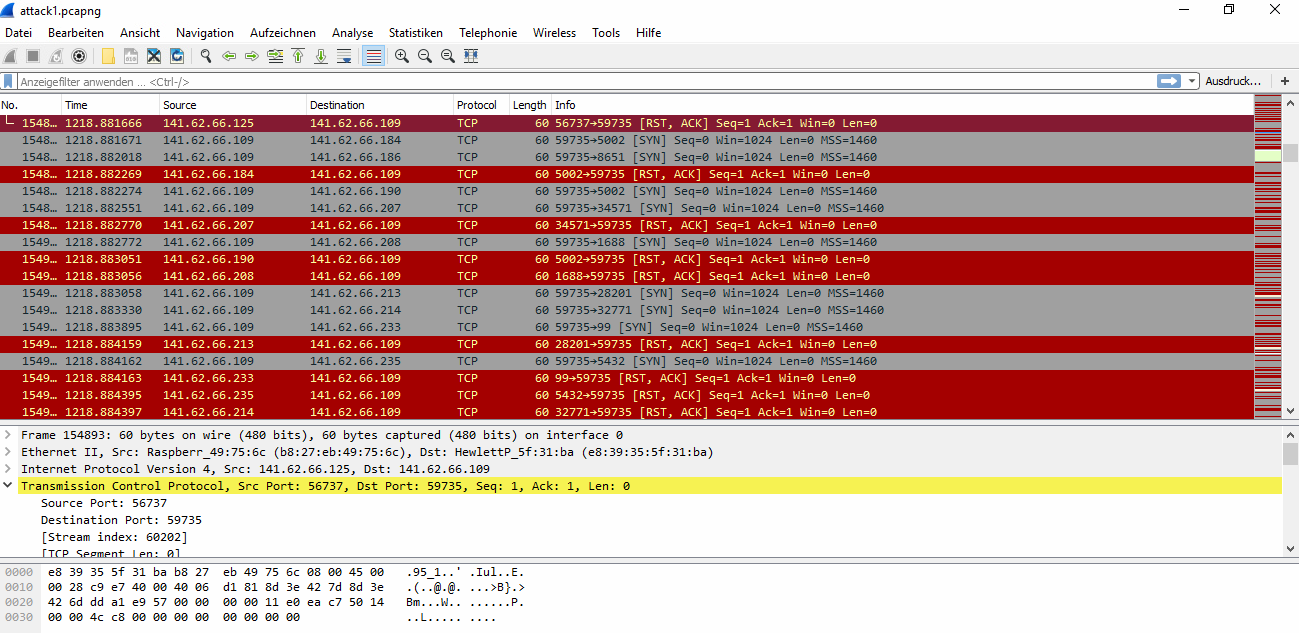
\includegraphics[width=1.0\textwidth]{pics/latex/tcpsynscan.png}
	\caption{Wireshark Logo}
	\label{fig:wiresharklogo}
\end{figure}

Das passiert im alert.log, wenn man Port 0 scannt (sehr typisch bei einem NMAP Port Scan Port 0 mit anzugeben):
\begin{lstlisting}
11/11-11:26:43.073895  [**] [1:524:8] BAD-TRAFFIC tcp port 0 traffic [**]
[Classification: Misc activity] [Priority: 3] {TCP} 141.62.66.190:41557 ->
141.62.66.111:0
11/11-11:26:43.074293  [**] [1:524:8] BAD-TRAFFIC tcp port 0 traffic [**]
[Classification: Misc activity] [Priority: 3] {TCP} 141.62.66.111:0 ->
141.62.66.190:41557
\end{lstlisting}

\newpage
\section{Teil 2 - IDS}
	
	
\subsection{Snort Regeln}

Öffnen der rules-Datei:
\begin{lstlisting}
sudo gedit /etc/snort/rules
\end{lstlisting}

Eintragen der neuen Regeln:

\iffalse
erste rule funktioniert nicht?! Nur abgeschrieben aus unserer Rules Datei. Keine Message aus alert.log gefunden.
\fi

\begin{lstlisting}
alert tcp any any -> any 111 
(flags: S; msg: "Possible SYN FIN scan"; sid:10000001;)
alert tcp any any -> any 111
(msg: "String istestlabor detected"; content:"istestlabor" sid:10000002;)
\end{lstlisting}

\begin{itemize}
\item tcp/udp: Gibt an, welcher Pakettyp verwendet wird.

\iffalse
Hier fehlt noch die genauere Beschreibung der einzelnen Attribute der Rule.
\fi

\item flags: S steht für SYN Pakete. (Siehe Three-Way-Handshake).\\
Es können auch andere Pakete selektiert werden, auf die reagiert werden soll.
\item msg: Gibt an, welche Nachricht im alert.log erscheinen soll, falls ein Muster detektiert wird.
\item content: Gibt an, auf welchen String reagiert werden soll.
\item sid: ist ein Akronym für Snort ID.  Jeder Snort Regelsatz hat eine einzigartige ID die es Output Modulen oder Log Scannern ermöglicht, die Regel die den Alarm ausgelöst hat zu identifizieren. 
\end{itemize}

Getestet wurde das ganze in dem wir eine FTP Verbindung zu einem anderen Client aufgenommen haben und als User und Passwort istestlabor eingetragen haben.
Die andere Rule wurde durch den Port Scan des Dozenten ausgelöst.

Dannach haben wir kontrolliert, ob die Regel auch tatsächlich funktioniert:

\begin{lstlisting}
sudo gedit /var/log/snort/alert.log
\end{lstlisting}

\begin{lstlisting}
11/11-11:54:44.087925  [**] [1:1000002:0] String istestlabor detected [**]
[Priority: 0] {TCP} 141.62.66.104:53724 -> 141.62.66.103:21
11/11-12:06:35.235065  [**] [1:10000001:0] Possible SYN FIN Scan [**]
[Priority: 0] {TCP} 141.62.66.190:56276 -> 141.62.66.102:111
\end{lstlisting}

\end{document}          